\section{COUPLED FIELDS ANALYSIS} \label{ch_5.4}
\normalsize{In the above chapter, it was concluded that complex coupled phenomena such as temperature and displacement dependant contacts. To understand the coupling method and its mathematical implications, a little introduction to coupling will be done.}
\subsection{Introduction to coupled fields analysis}
\normalsize{There are many different methods for multiphysics coupling. This idea of coupling fields is to consider the effect of field A on field B and vice-versa using coupling terms.}
\\
\begin{figure}[!ht]
    \label{fig_5_20}
    \centering
    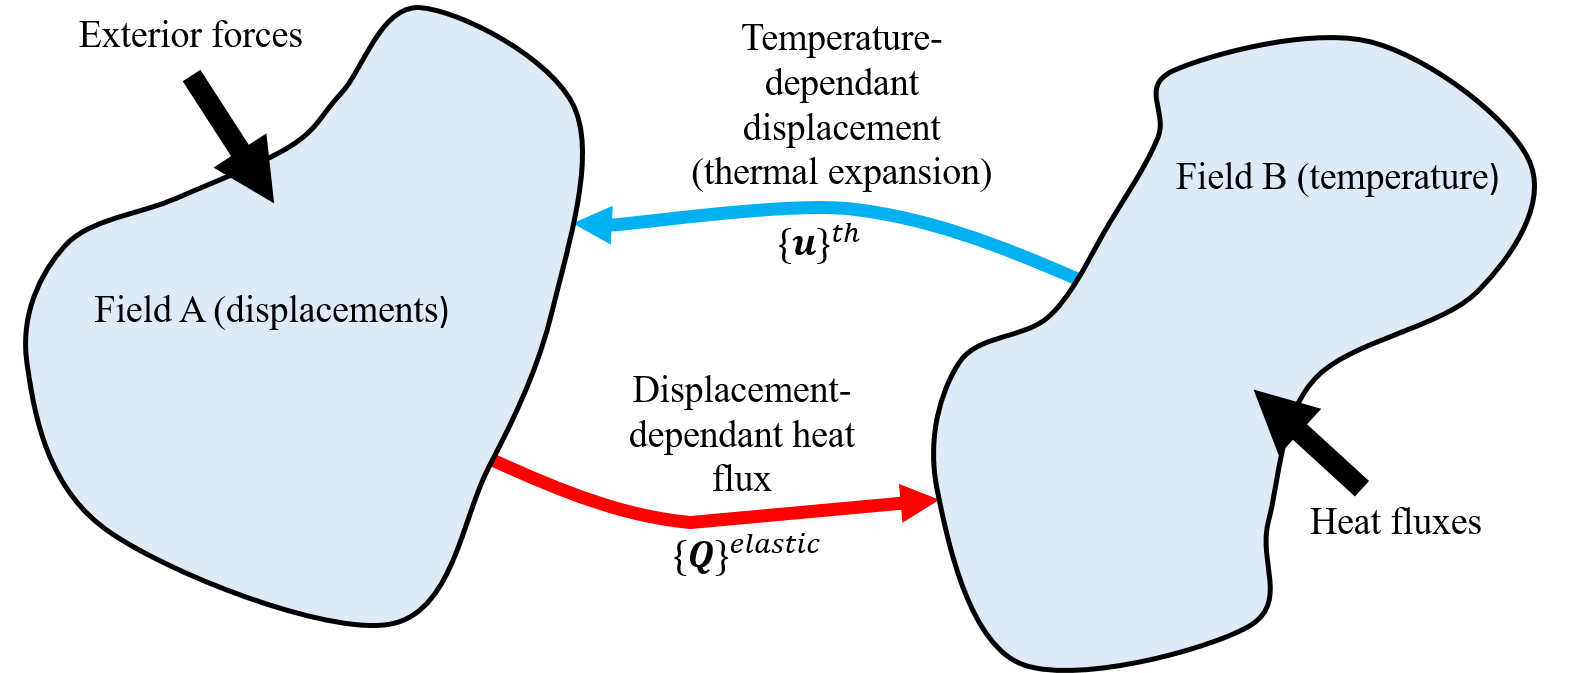
\includegraphics[width=1\textwidth]{figures/patateCoupling.png}
    \caption{\it Fields coupling.}
\end{figure}
\\
\normalsize{The coupling can be made of two different levels, the weak coupling (vector coupling) and the strong coupling (matrix coupling). The vector coupling is generally less computationally expensive. It works by adding to the right-hand side of the equation a coupling vector.}
\\

\begin{gather}
    \begin{bmatrix} K[1,1] & 0 \\ 0 & K[2,2] \end{bmatrix}
    \begin{Bmatrix} \{Displacement \ field\} \\ \{Temperature \ field\} \end{Bmatrix}
    =
    \begin{Bmatrix} \{Forces\}+\{Forces\}_{thermal} \\ \{Heat \ fluxes\}+\{Heat \ fluxes\}_{th. elastic} \end{Bmatrix}
    \label{eq:coupling}
\end{gather}
\\
\normalsize{\indent This method is less computationally expensive since the coupling is done ba adding the coupling vector. The system matrix is diagonal, meaning that it is possible to decouple the calculation of the displacement field and the temperature field and create two subproblems such that:}
%\\
%\begin{gather}
%    K[1,1] \{Displacement \ field\} = \{Forces\}+\{Forces\}_{thermal}
%\end{gather}
%\normalsize{and the other}
%\begin{gather}
%    K[1,1] \{Temperature \ field\} = {Heat \ fluxes\}+\{Heat \ fluxes\}_{th. elastic}
%\end{gather}
\\
\normalsize{\indent This also means that the fields are NOT calculated at the same time but rather one after the other. The method while taking less storage space requries more steps. Another way to couple the fields is using the strong coupling (matrix coupling). In this method, the fields are not longer coupled using a coupling vector but rather directly in the system matrix by introducing off-diagonal coupling terms {\bfseries K[1,2]} and {\bfseries K[2,1]}. Those terms allows a direct coupling of the fields as well as simultaneous calculations of the solution vector. This method is computationally expensive and will require more storage space but less steps.}
\\
\begin{gather}
    \begin{bmatrix} K[1,1] & K[1,2] \\ K[2,1] & K[2,2] \end{bmatrix}
    \begin{Bmatrix} \{Displacement \ field\} \\ \{Temperature \ field\} \end{Bmatrix}
    =
    \begin{Bmatrix} \{Forces\} \\ \{Heat \ fluxes\} \end{Bmatrix}
    \label{eq:coupling3}
\end{gather}
\\
caca
\subsection{Static thermal-structural analysis of the tile assembly}